\chapter{Ejercicio juego del pañuelo} \label{gripper}
En este capítulo se expone como ha sido el desarrollo del ejercicio del juego del pañuelo. Primero hablaremos del enunciado del ejercicio, seguidamente se muestra como ha sido su implementación, las herramientas se han utilizado, prototipos y como se ha llevado a cabo el ejercicio. Finalmente se ofrecen dos soluciones de referencia que resuelven el ejercicio en Kibotics.

\section{Enunciado}
El propósito de este ejercicio es crear un nuevo ejercicio en Kibotics con un nuevo robot que sea capaz de coger objetos y moverlos por el escenario. El nuevo robot debe tener pinzas móviles para atrapar otros objetos. 

El juego del pañuelo es muy popular entre los más pequeños y también en el mundo de la robótica. En las competiciones de robots este juego consiste en programar un sigue líneas. El robot debe recorrer un circuito y el robot debe ser capaz coger una lata que obstaculiza el camino  y volver con ella a la posición de salida. En la Figura 6.1 a y 6.2 b podemos ver como es este juego en competiciones de robótica.

\begin{figure}[H]
  \begin{subfigure}[b]{0.5\textwidth}
  \centering
    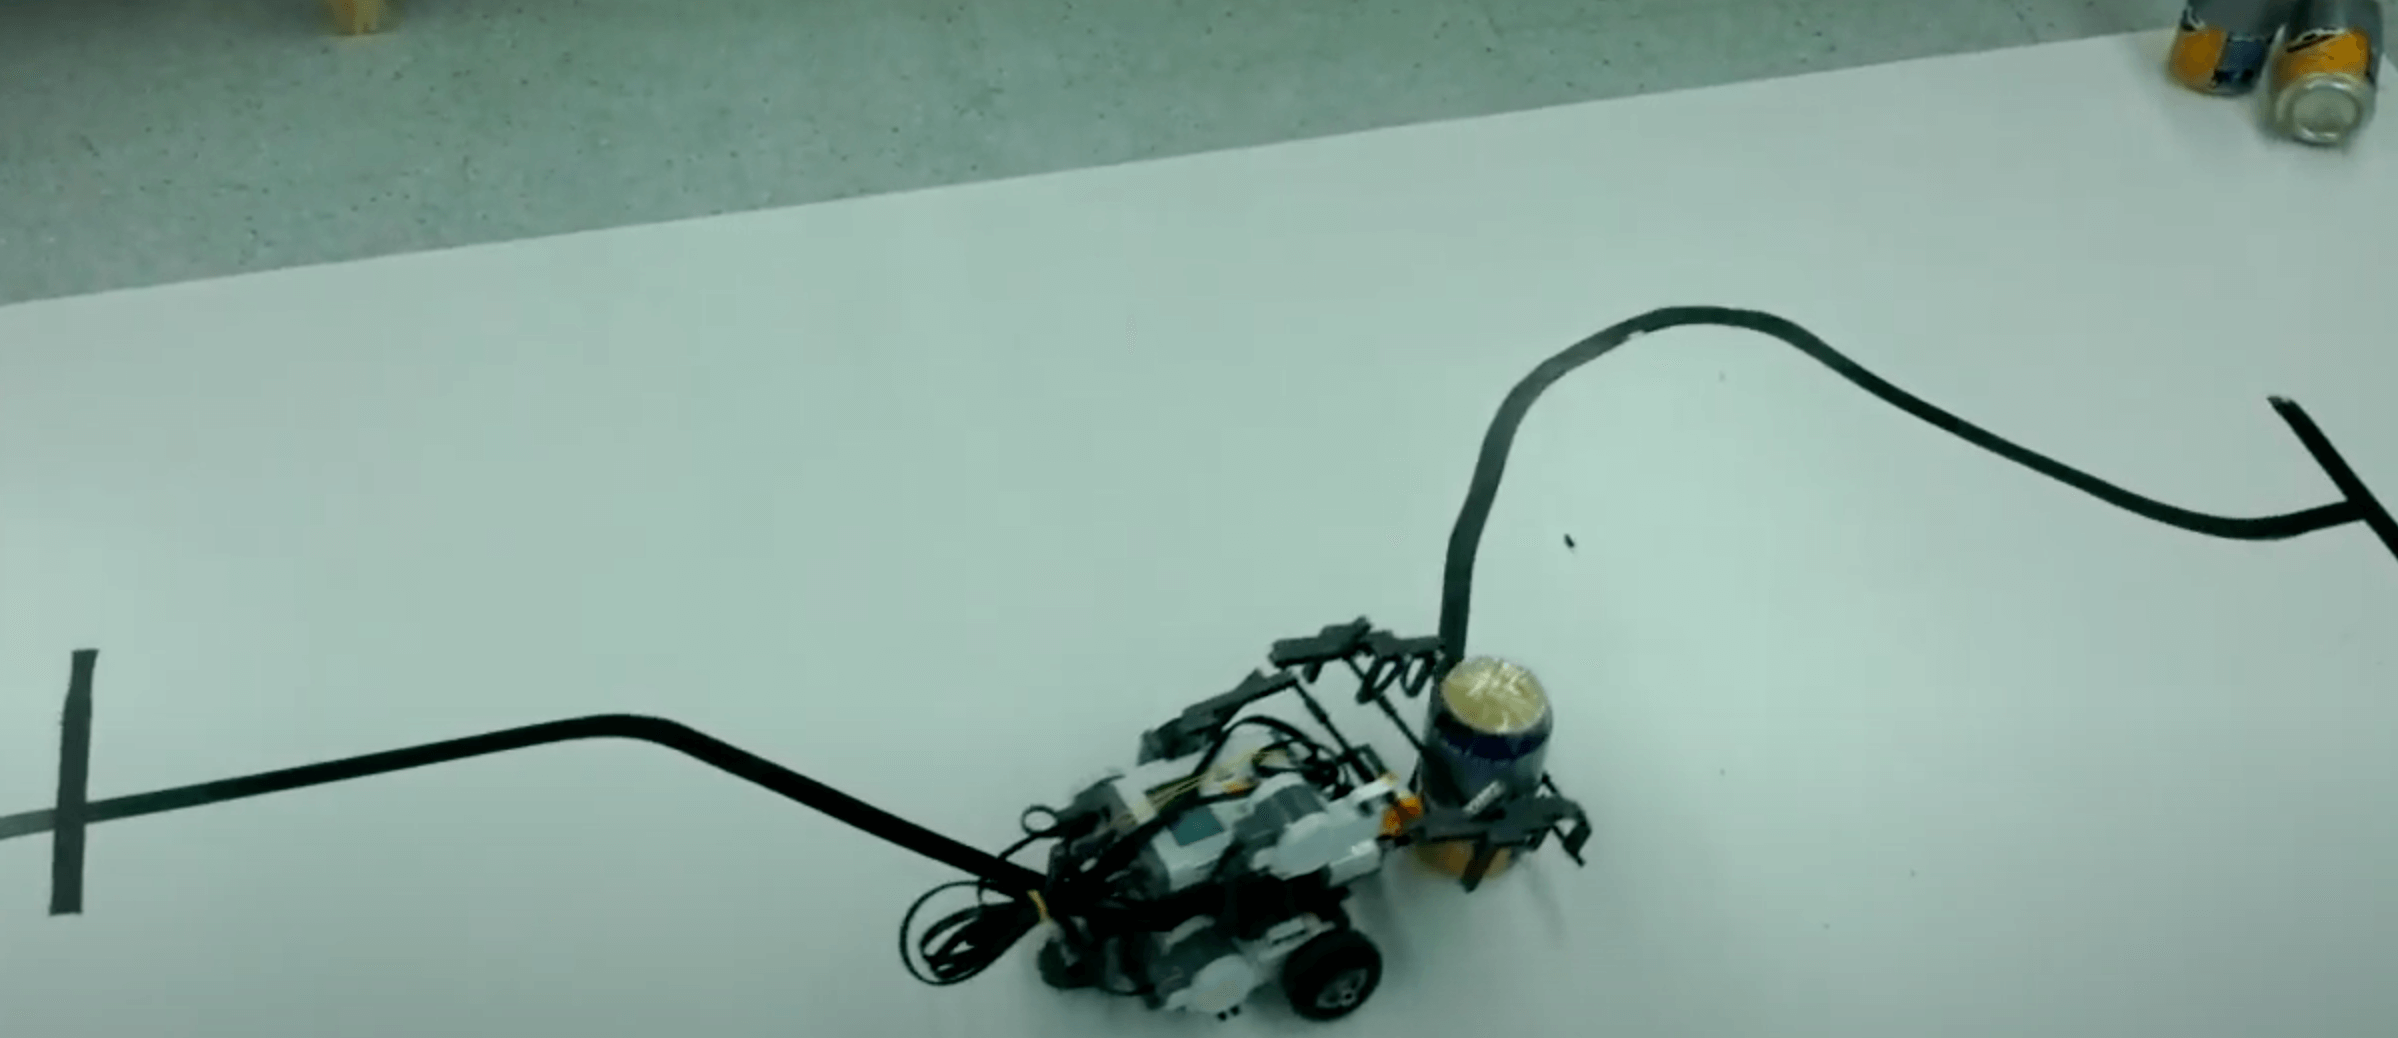
\includegraphics[width=0.95\textwidth, height=0.4\textwidth]{chapters/images/jp.png}
    \caption{Juego del pañuelo con un robot \footnote{https://www.youtube.com/watch?v=FsS2CSudl7c}}
    \label{fig:f1}
  \end{subfigure}
  \hfill
  \begin{subfigure}[b]{0.5\textwidth}
  \centering
    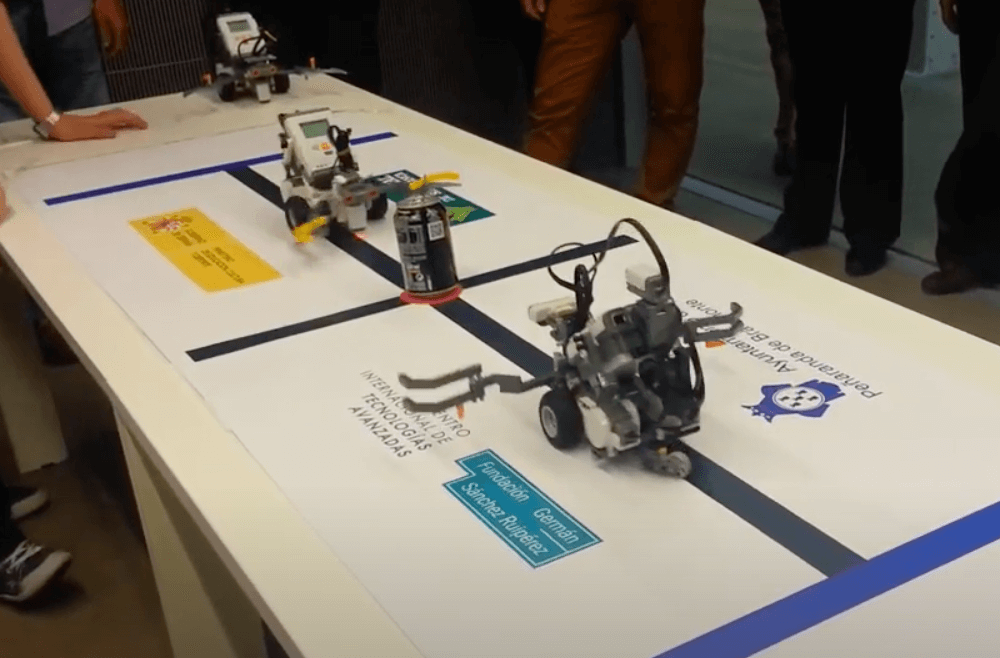
\includegraphics[width=0.95\textwidth, height=0.4\textwidth]{chapters/images/jp2.png}
    \caption{Juego del pañuelo multirobot \footnote{https://www.youtube.com/watch?v=6T\_Ua\-TaB6Q}}
    \label{fig:f2}
  \end{subfigure}
  \caption{Juego del Pañuelo en competiciones robóticas}

\end{figure}

 
El alumno deberá programar en Python o en Scratch un algoritmo que permita que el Mbot Pinza avance siguiendo la linea negra del circuito hasta que se encuentre a poca distancia de la lata, una vez se encuentre enfrente de la lata, tu robot debe cerrar las pinzas y dar media vuelta para volver a la casilla de salida y  llevar consigo la lata en todo momento. Gracias a un evaluador automático vamos a obtener la puntuación, esta depende del porcentaje de circuito recorrido y si se lleva o no la lata entre las pinzas.

\section{Desarrollo del ejercicio}

Para que nuestro ejercicio sea acorde con el juego del pañuelo que conocemos todos y con las competiciones actuales, necesitamos hacer un robot con pinzas, una lata  y un circuito.
Se investigó un prototipo que estaba realizado en A-Frame nativo, (HTML5, JavaScript y la librería de A-Frame) sin Websim.
En este primer prototipo se cogía el modelo .gltf del Mbot que ya se usaba en Kibotics para algunos ejercicios y lo representaba en la escena, el robot se movía con eventos de teclado desde JavaScript que hacían que este cambiara su posición. Las pinzas que eran dos octaedros a los lados del robot. Estas pinzas estaban creadas con a-box y eran  independientes del robot. Con este prototipo se estudió el movimiento de las pinzas con respecto a la posición del robot. En el código JavaScript era muy complejo y dependía de la actualización continua de la posición y se encontraron muchas dificultades a la hora de realizar giros del robot con las pinzas dado que estas estaban definidas por el centro de masas y al rotarlas había que hacerlo con funciones senoidales para que se movieran en concordancia con la rotación del robot. En estos vídeos \footnote{https://www.youtube.com/watch?v=BpAujxcWx-Y}\footnote{https://www.youtube.com/watch?v=w5plHB\_4G7Y} se puede ver el prototipo y los problemas con el giro.

En este trabajo fin de grado ese prototipo se llevó Websim pero no funcionaba bien. Esta dependencia continua de la posición del robot con respecto a las pinzas y la lata con el cierre de las pinzas era muy compleja y muy poco realista. En este video  \footnote{https://www.youtube.com/watch?v=eVM9n4mziTQ\&t=46s} se puede ver como era el funcionamiento en Websim con el JavaScript del primer prototipo.  


La idea principal de este ejercicio era que el robot pudiera coger con las pinzas una lata de la forma más natural posible. Las pinzas había que hacerlas dependientes del robot para que su movimiento y los giros sean coherentes. 

Primero se se creó el modelo 3D de una lata en Blender y con  GIMP un programa de edición de imágenes gratuito y multiplataforma se diseño la imagen .png del circuito. Para el robot base se uso el modelo base del Mbot que ya teniamos su  .gltf, para que fuera diferente a los anteriores que se usaban en la plataforma se cambió el color del robot desde Blender con tonos amarillos y azules.
Los objetos se añadieron con sus respectivos modeos al fichero de configuración.

 Para que las pinzas fueran dependientes del robot desde el fichero de configuración se definieron como \textit{childs} del objeto Mbot base, de esta forma las pinzas y el robot forman un mismo objeto y se mueven a la vez.

Ala hora de crear la escena en el fichero de configuración de este ejercicio gripper.json se tuvo que añadir el atributo ``renderer":``colorManagement: true"  para que los colores en Websim, fueran los mimos que se habían diseñado en Blender, sino los modelos se veían más oscuros. 

\begin{figure}[H]
  \begin{subfigure}[b]{0.5\textwidth}
  \centering
    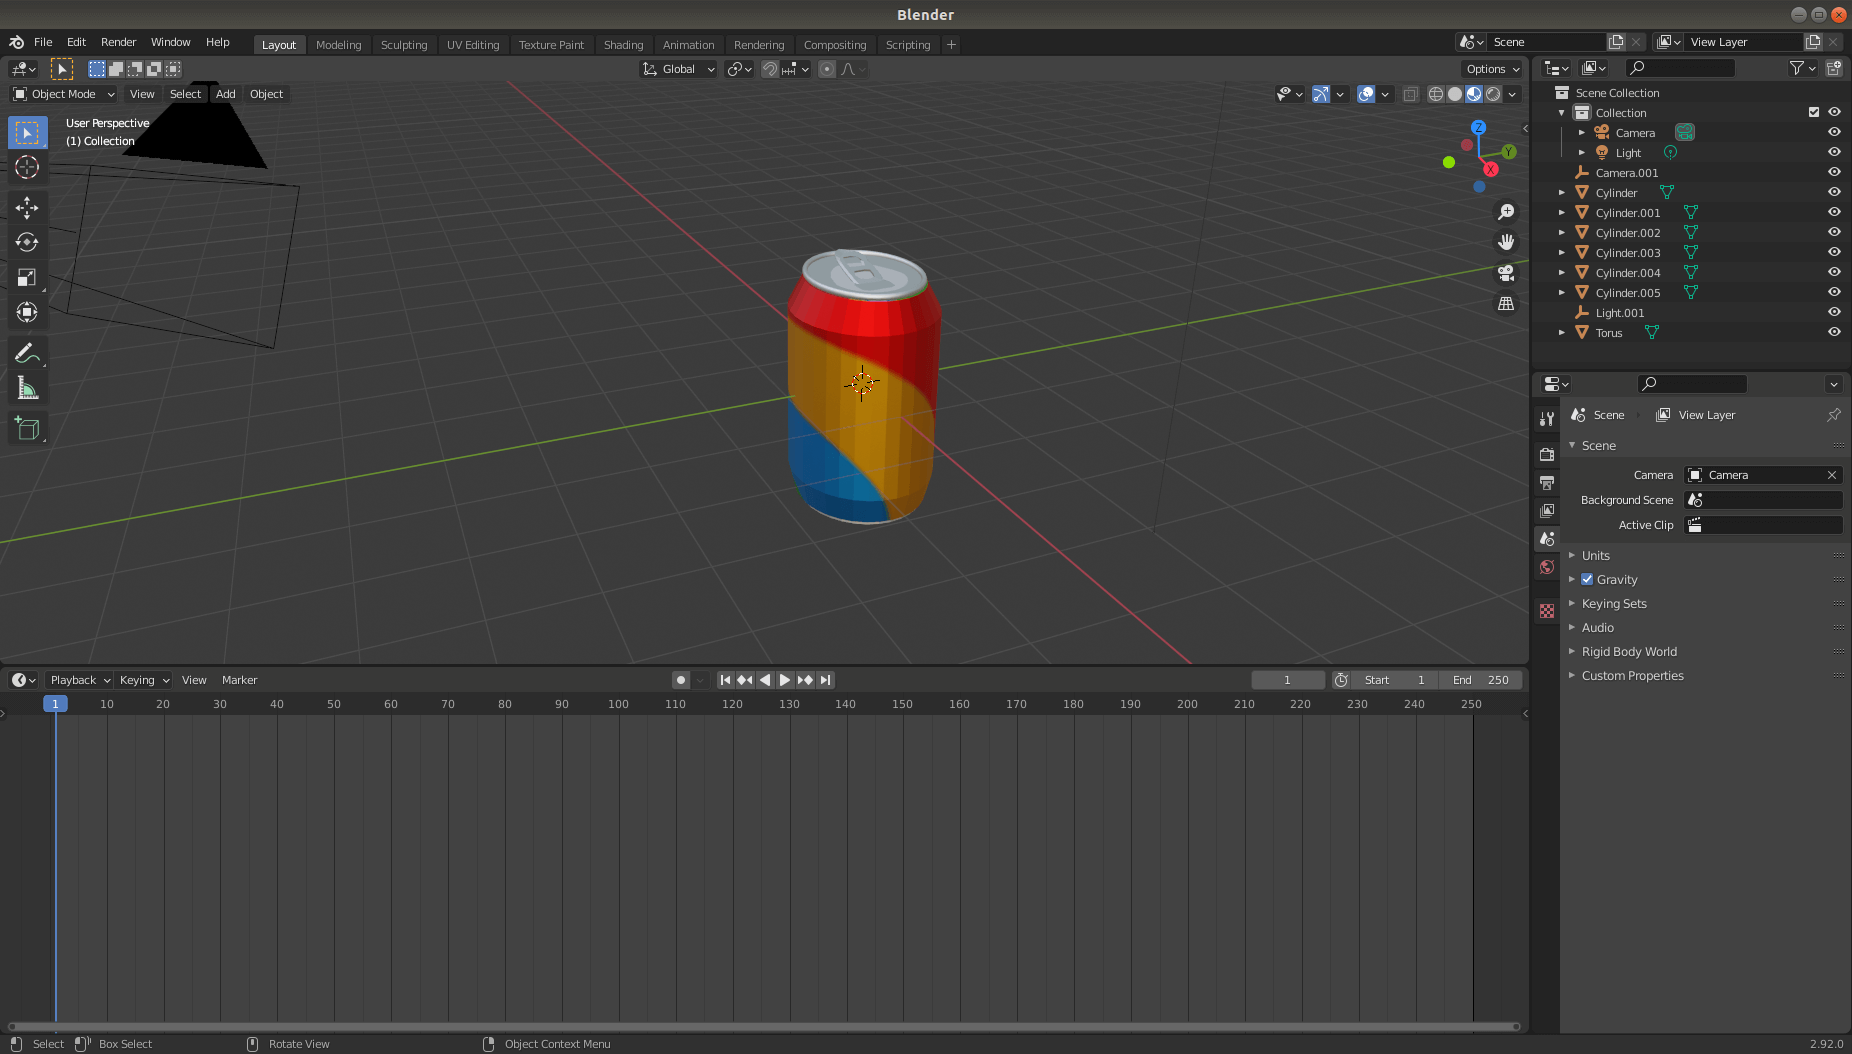
\includegraphics[width=0.8\textwidth, height=0.5\textwidth]{chapters/images/lata.png}
    \caption{Modelo lata}
    \label{fig:f1}
  \end{subfigure}
  \hfill
  \begin{subfigure}[b]{0.5\textwidth}
  \centering
    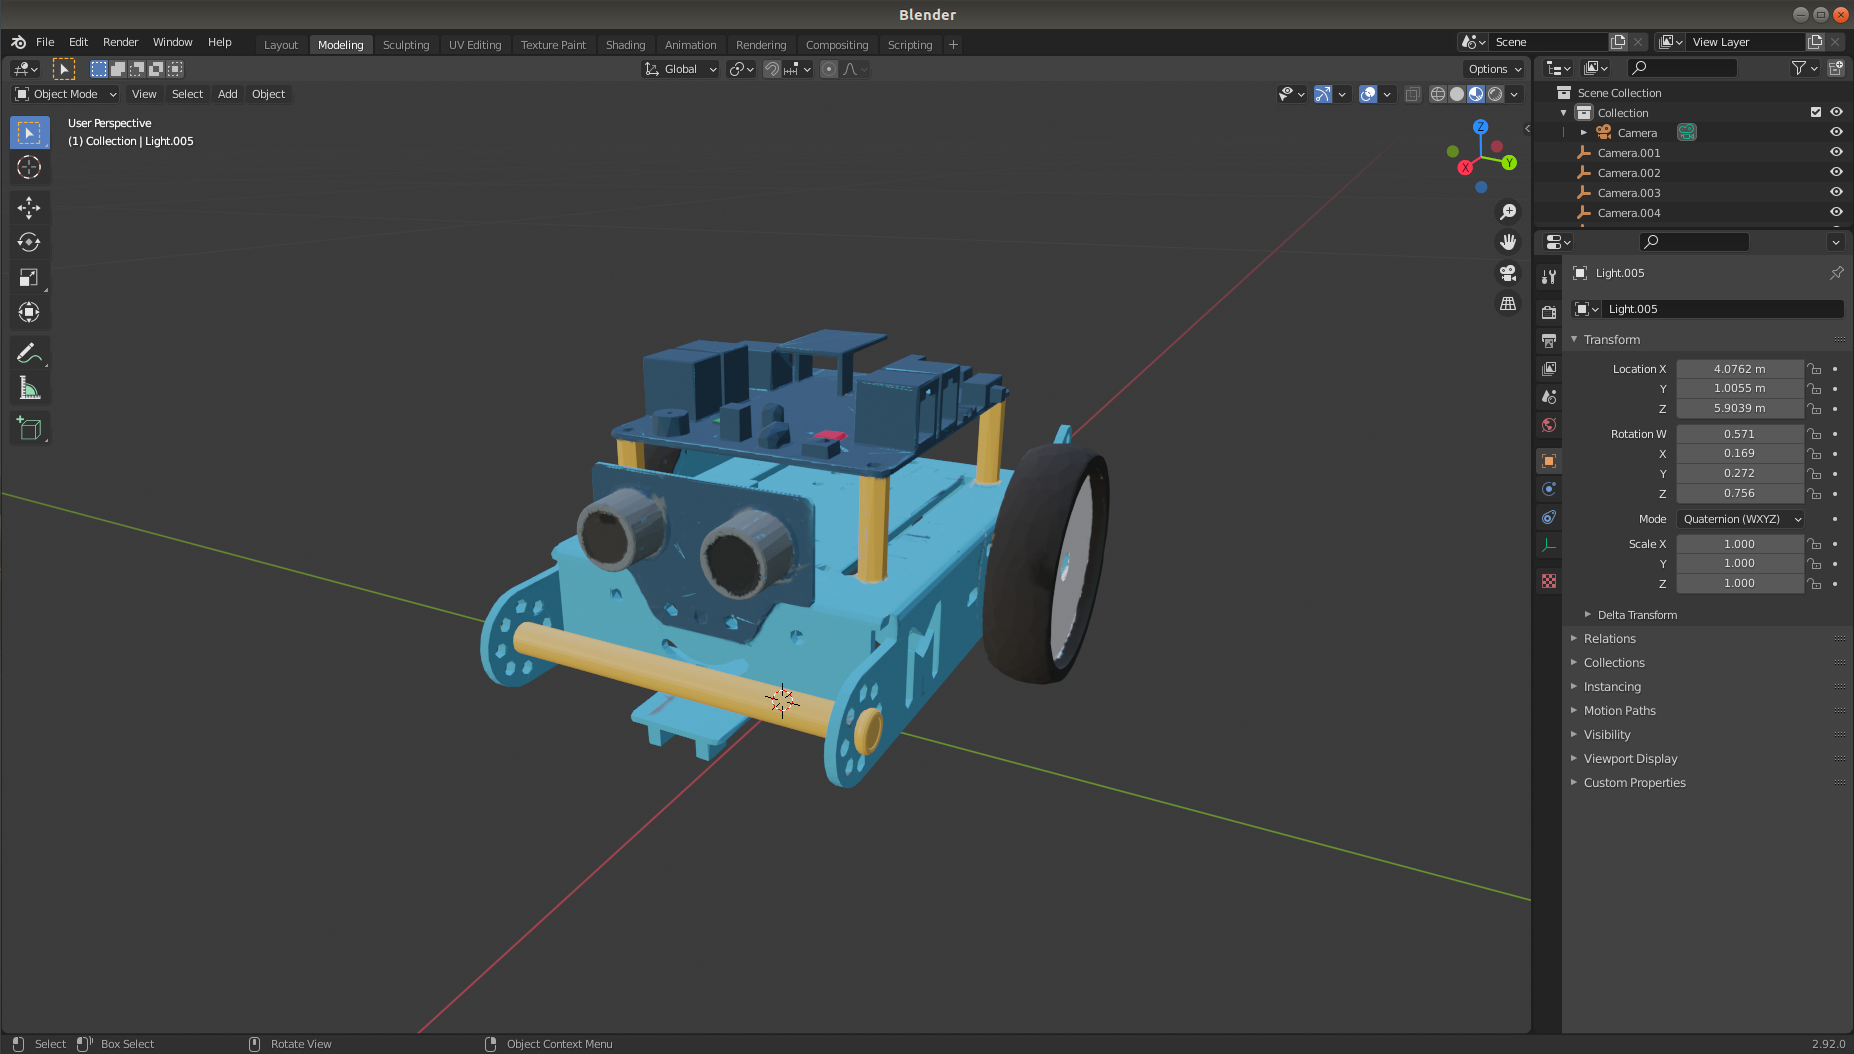
\includegraphics[width=0.8\textwidth, height=0.5\textwidth]{chapters/images/mbotbase.png}
	\caption{Modelo Mbot cambiado de color}    
    \label{fig:f2}
 
  \end{subfigure}
  \caption{Modelos en Blender}
\end{figure}

\begin{figure}[H]
  \centering
 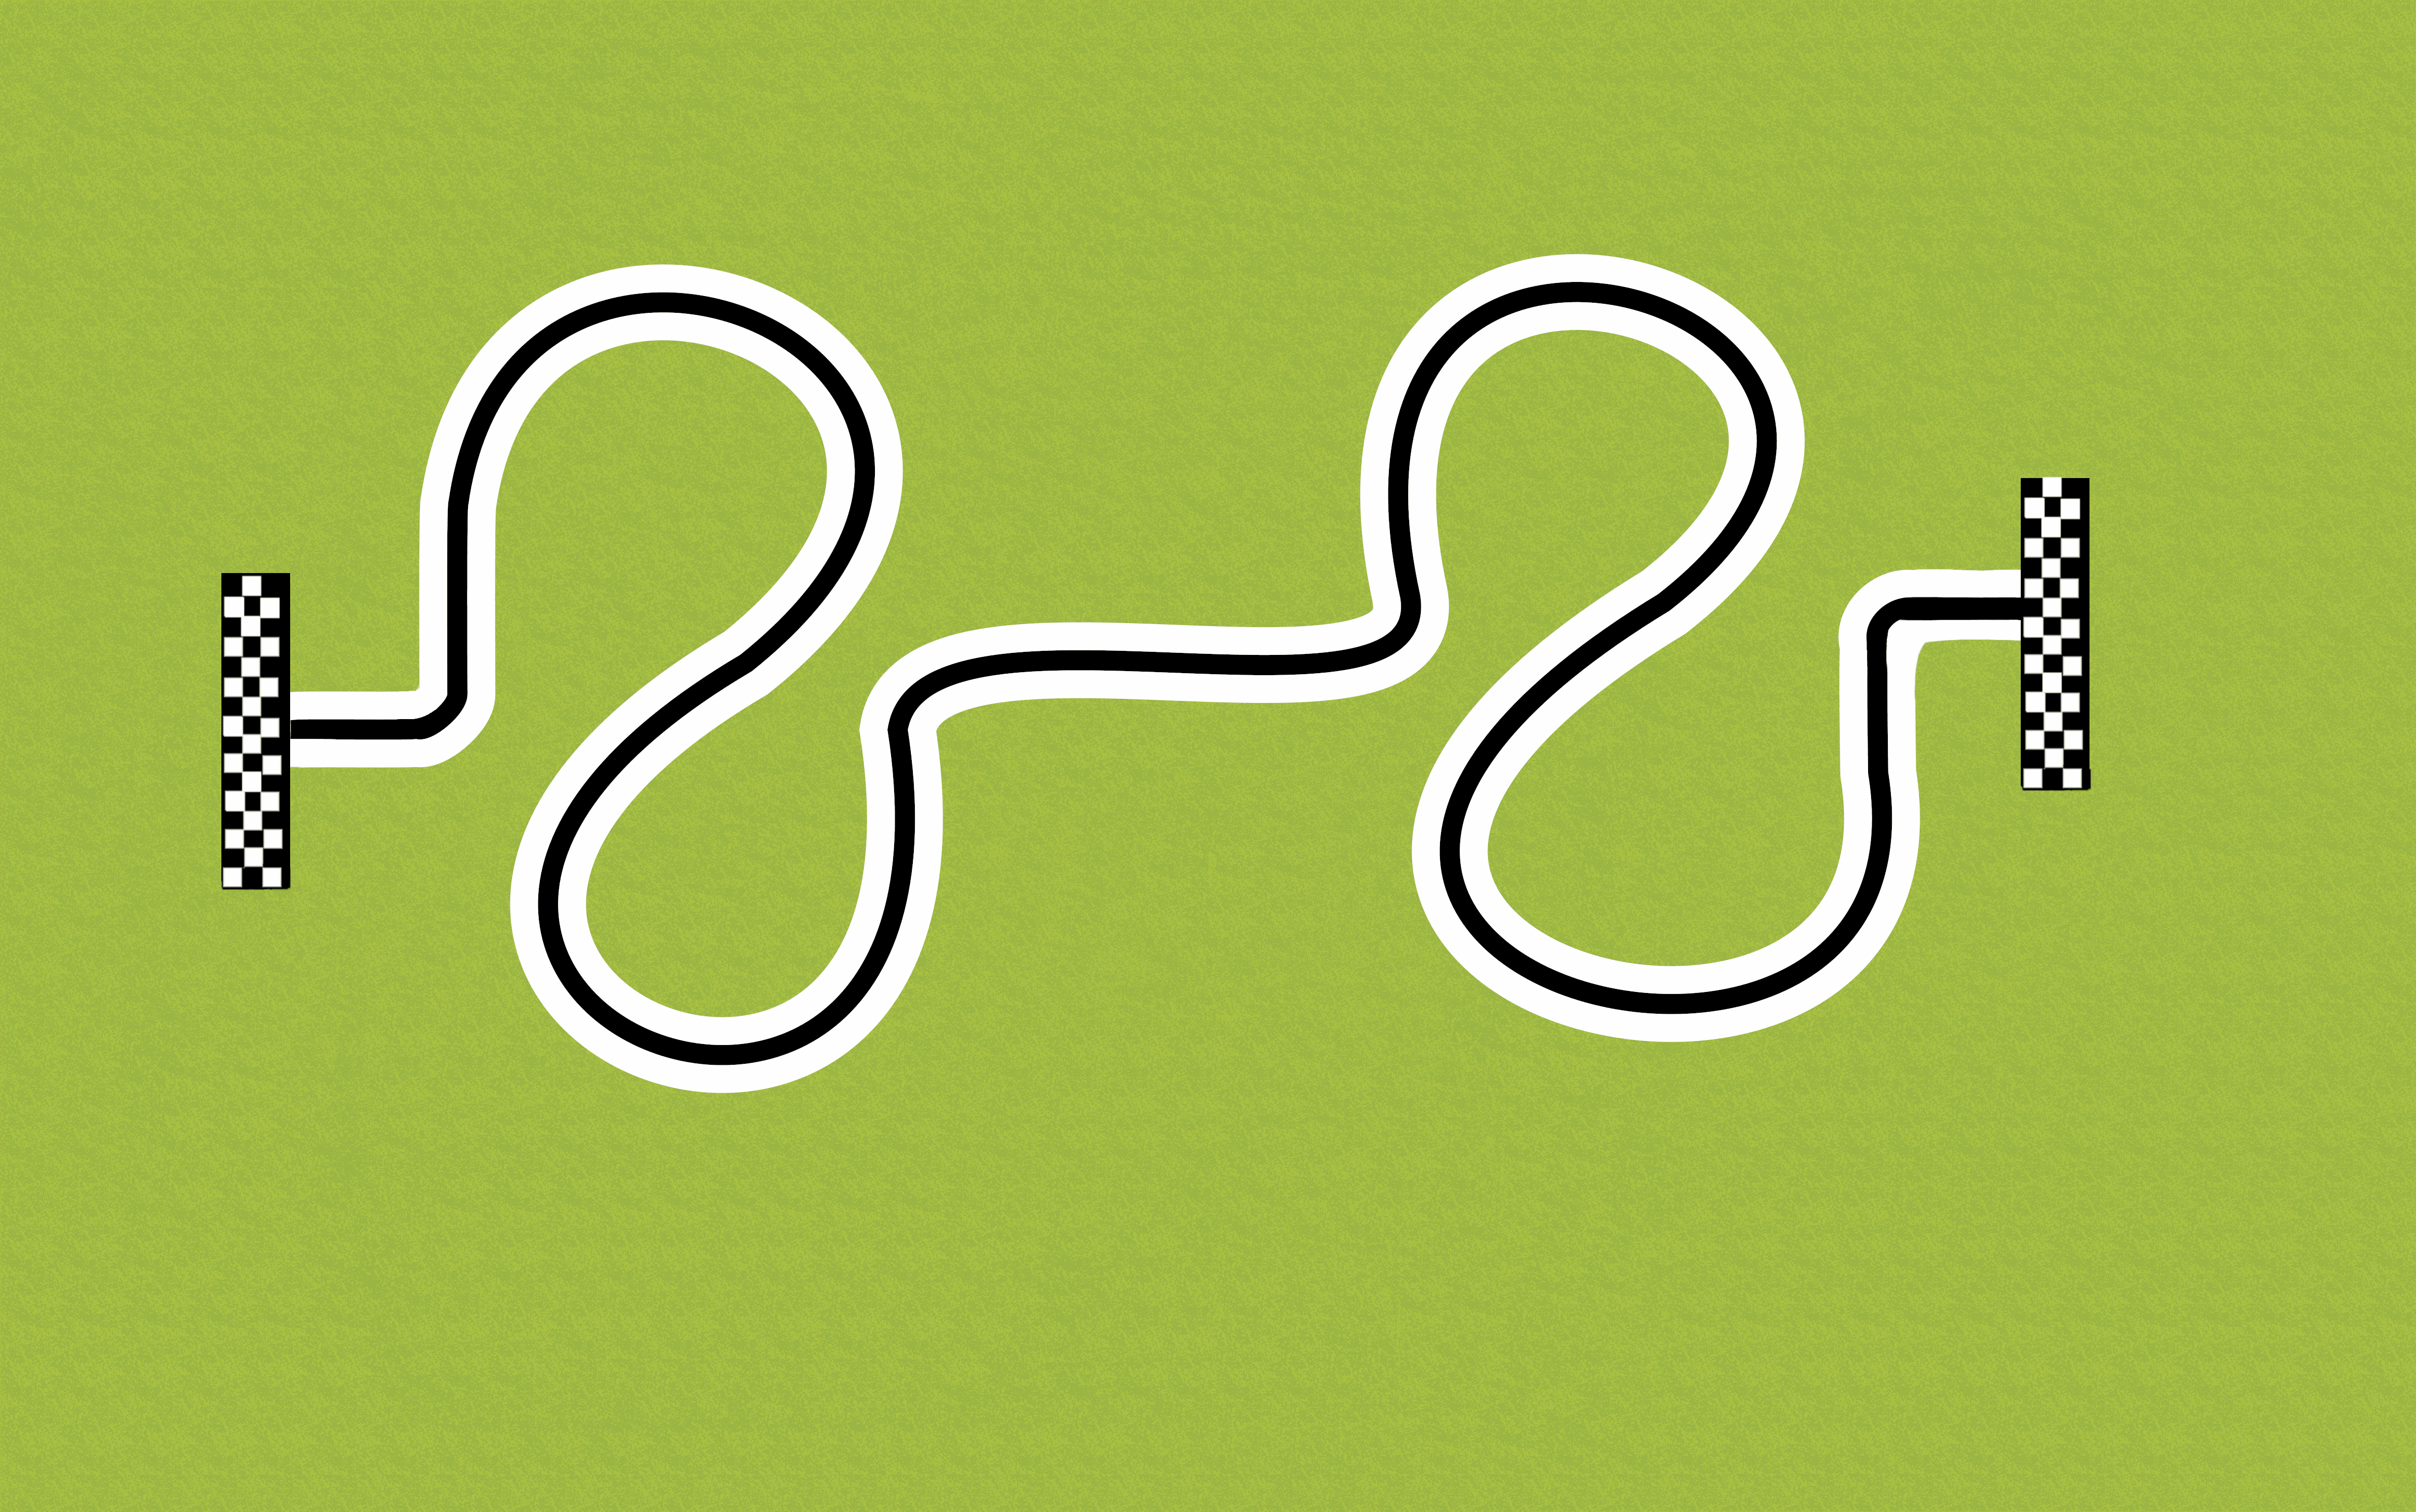
\includegraphics[width=0.7\textwidth, height=0.4\textwidth]{chapters/images/handkerchief.png}
  \caption{Circuito diseñado en GIMP del juego del pañuelo}
\end{figure}

Para las pinzas  primero se implementaron ortoedros gracias a la etiqueta  \textless box \textgreater de A-Frame. Pero finalmente se cambiaron por un modelo más moderno diseñado en Blender.

\begin{figure}[H]
  \centering
 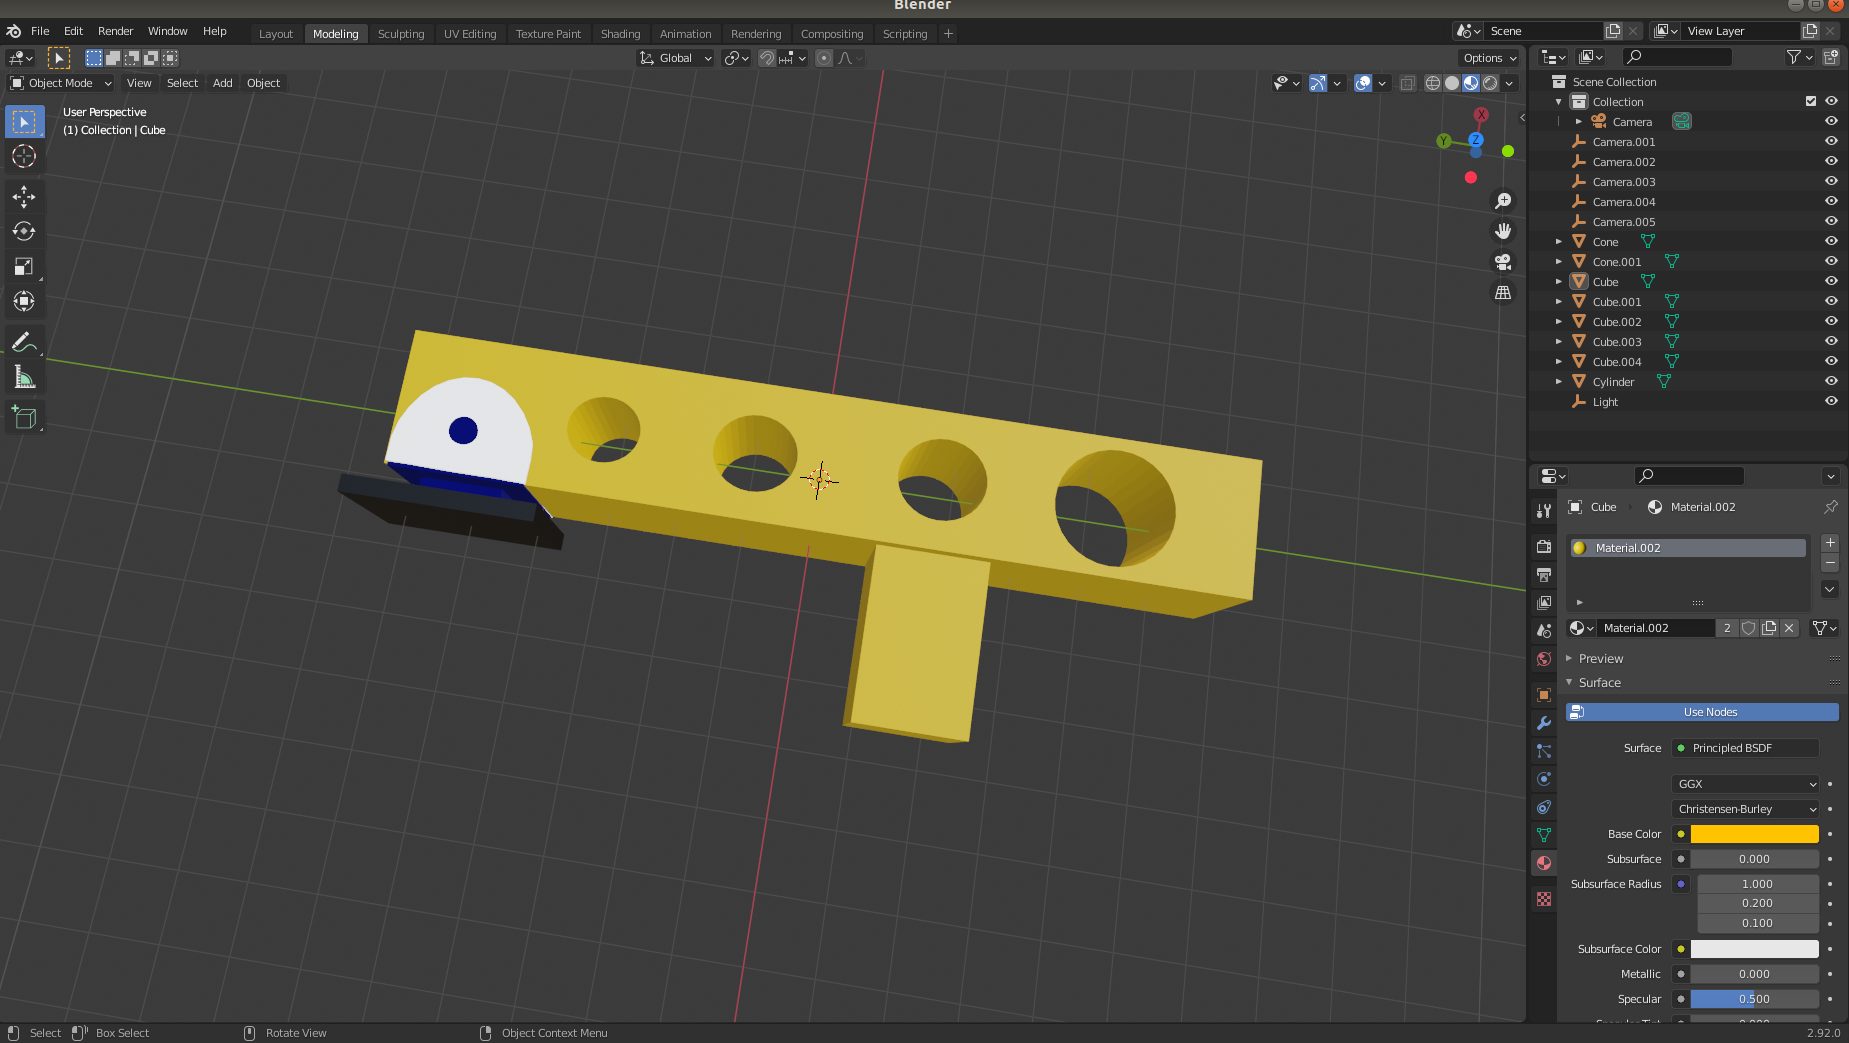
\includegraphics[width=0.8\textwidth, height=0.5\textwidth]{chapters/images/pinza.png}
  \caption{Modelos de las pinzas en Blender}
\end{figure}

Una vez con todo el escenario creado se estudió la posibilidad de que ajustando  las mallas de colisión de las pinzas se pudiera atrapar una lata con la fuerza que ejercieran las pinzas al cerrarse. 
Las mallas de colisión son las líneas rojas que delimitan el entorno de un objeto y permiten definir una forma física alrededor de modelos personalizados. De esta forma funcionarán mejor y se comportarán con mayor realismo.

En A-Frame existen dos tipos de cuerpos de los objetos: dynamic\-body y static\-body. Un objeto con dynamic-body  se mueve libremente. Los cuerpos dinámicos tienen masa, chocan con otros objetos, rebotan o se ralentizan durante las colisiones y caen si la gravedad está habilitada.
Los cuerpos estáticos son objetos animados o de posición fija. Otros objetos pueden chocar con cuerpos estáticos, pero los cuerpos estáticos en sí mismos no se ven afectados por la gravedad y las colisiones.

El robot se definió como un cuerpo dinámico mientras que las palas de las pinzas eran cuerpos estáticos, de esta forma, las palas pueden estar elevadas del suelo y no les afecta  radicalmente las colisiones que pueda tener con la lata a la hora de cerrarse.  La lata en cambio es un objeto dinámico.

Cada pala se define de la siguiente forma: 

\begin{lstlisting}         
         {
              "tag": "a-box",

              "attr": {
                "id":"gripper-right",
		        "gltf-model":"/static/websim/assets/models/gripper.gltf",
                "position": { "x":0.033, "y":0, "z":-0.05},
                "scale": { "x":0.005, "y":0.005, "z":0.006},
                "rotation": { "x": 0, "y":8, "z":0},
 			  "body":{"type": "static", "mass": 1, "shape":"none"},
                             "shape__main":{"shape": "box",
			                "halfExtents": "1.5 1.5 6.5",
                              "offset": "0 0 0"},
		       "shape__handle":{"shape": "box",
                              "halfExtents": "1.5 1 1",
                              "offset": "-2.2 -0.2 1.75"}
               }
               [...]
\end{lstlisting}


La malla de colisión se define por \textit{shape\_main y shape\_handle}. En body se pone a ``none'' la malla de colisión que viene por defecto para poder ajustarla a mano.
\textit{Shape\_main} es la malla de colisión principal en la que se puede elegir la forma\textit{shape}, lo que ocupa \textit{halfExtents} y se puede desplazar del centro del objeto \textit{offset}. Esto nos permite hacer la malla de colisión más grande o más pequeña que las dimensiones de nuestro objeto. \textit{ Shape\_handle} nos permite añadir una malla de colisión extra independientemente de si dentro de ese  objeto hay otro objeto o no. Esta malla de colision extra se define respecto a la malla de colisión shape\_ main. Ambas mallas de colision dependeran de la posición del objeto y se moverán lo mismo que él.

Los usuarios tienen que programar el Mbot para que este abra y cierre las pinzas cuando la lata esté cerca. Para ello, implementaron las funciones, closeGripper(), openGripper() y getObjectInGripper() en JavaScript para luego poder crear los bloques y funciones respectivas en Scratch y Python para que los usuarios puedan manejar todas las operaciones del robot. 
 
 En Scracth se crearon nuevos bloques en los Motores : Abrir pinza, Cerrar Pinza y Dame objeto en pinza.
 En Python  se crearon las nuevas funciones: HAL.abrir\_pinza(), HAL.cerrar\_pinza() y  HAL.dame\_objeto\_en\_pinza() que en el fondo todas ellas llaman a funciones en JavaScript para mover el robot.
 
\begin{lstlisting}
export async function closeGripper() {

    let thread = getThread(this.myRobotID);
    thread.blocking_instruction = true;
    let gripperLeft = document.querySelector("#gripper-left")
    let gripperLeftPos = gripperLeft.object3D.position
    let gripperRight = document.querySelector("#gripper-right")
    let gripperRightPos = gripperRight.object3D.position
    let val = 0.025
    while (getThread(this.myRobotID).status !== "RELOADING" && gripperLeftPos.x < -0.020 && gripperRightPos.x > 0.020) {
        val = val - 0.001
        await document.querySelector("#gripper-left").setAttribute('position', {x: -val, y:0 , z: -0.05})
        await document.querySelector("#gripper-right").setAttribute('position', {x: val, y:0 , z: -0.05})
        await this.sleep(0.2);
    }
    thread.blocking_instruction = false;
}

export function getObjectInGripper() {
    let distance = this.getDistance();
    if (distance < 1.5) {
        return 1;
    } else {
        return 0;
    }
}

export async function openGripper() {
    await document.querySelector("#gripper-left").setAttribute('position', {x: -0.030, y:0 , z: -0.05})
    await document.querySelector("#gripper-right").setAttribute('position', {x: 0.030, y:0 , z: -0.05})

}
\end{lstlisting}

 
En este punto la lata colisionaba con las mallas de las pinzas pero no se quedaba atrapada,  por eso se rotaron 8  grados en el eje y se ajustaron las físicas del mundo para que la lata no pudiera escaparse y el robot pudiera arrastrarla sin problema por el escenario.

Por útimo se hizo un evaluador automático para mostrar el porcenaje del circuito recorrido y unos iconos para indicar que la lata esta cogida o no, también se muestra y se guarda la puntuación total teniendo en cuenta el  porcentaje recorrido  y se suman 14 puntos si el robot lleva la lata y 20 puntos más si recorres todo el cicuito con ella. Esto se hizo en un fichero .js que se importa al ejercicio llamado gripper\_evaluator.js. En la Figura 6.5 se puede ver la rotación de las pinzas y la visualización del evaluador.

 \begin{figure}[H]
  \centering
 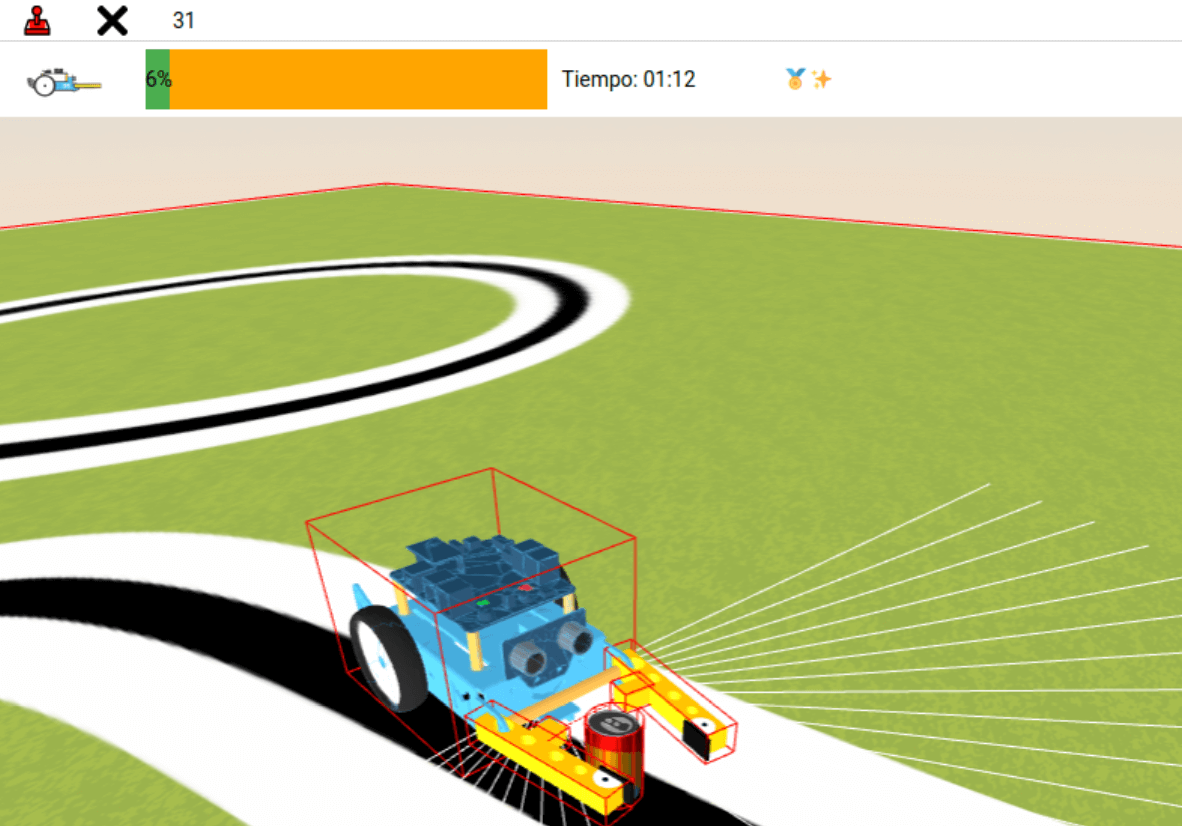
\includegraphics[width=0.8\textwidth, height=0.5\textwidth]{chapters/images/evaluadorpinza.png}
  \caption{Absorción por posición, el confeti es invisble cuando el robot pasa por encima.}
\end{figure}
Finalmente se añadió el nuevo ejercicio a Kibotics en su versión de Python y Scratch y se añadió la teoría relacionada con este ejercicio para facilitar su uso y aumentar los conocimientos de los usuarios.


\begin{figure}[H]
    \centering
    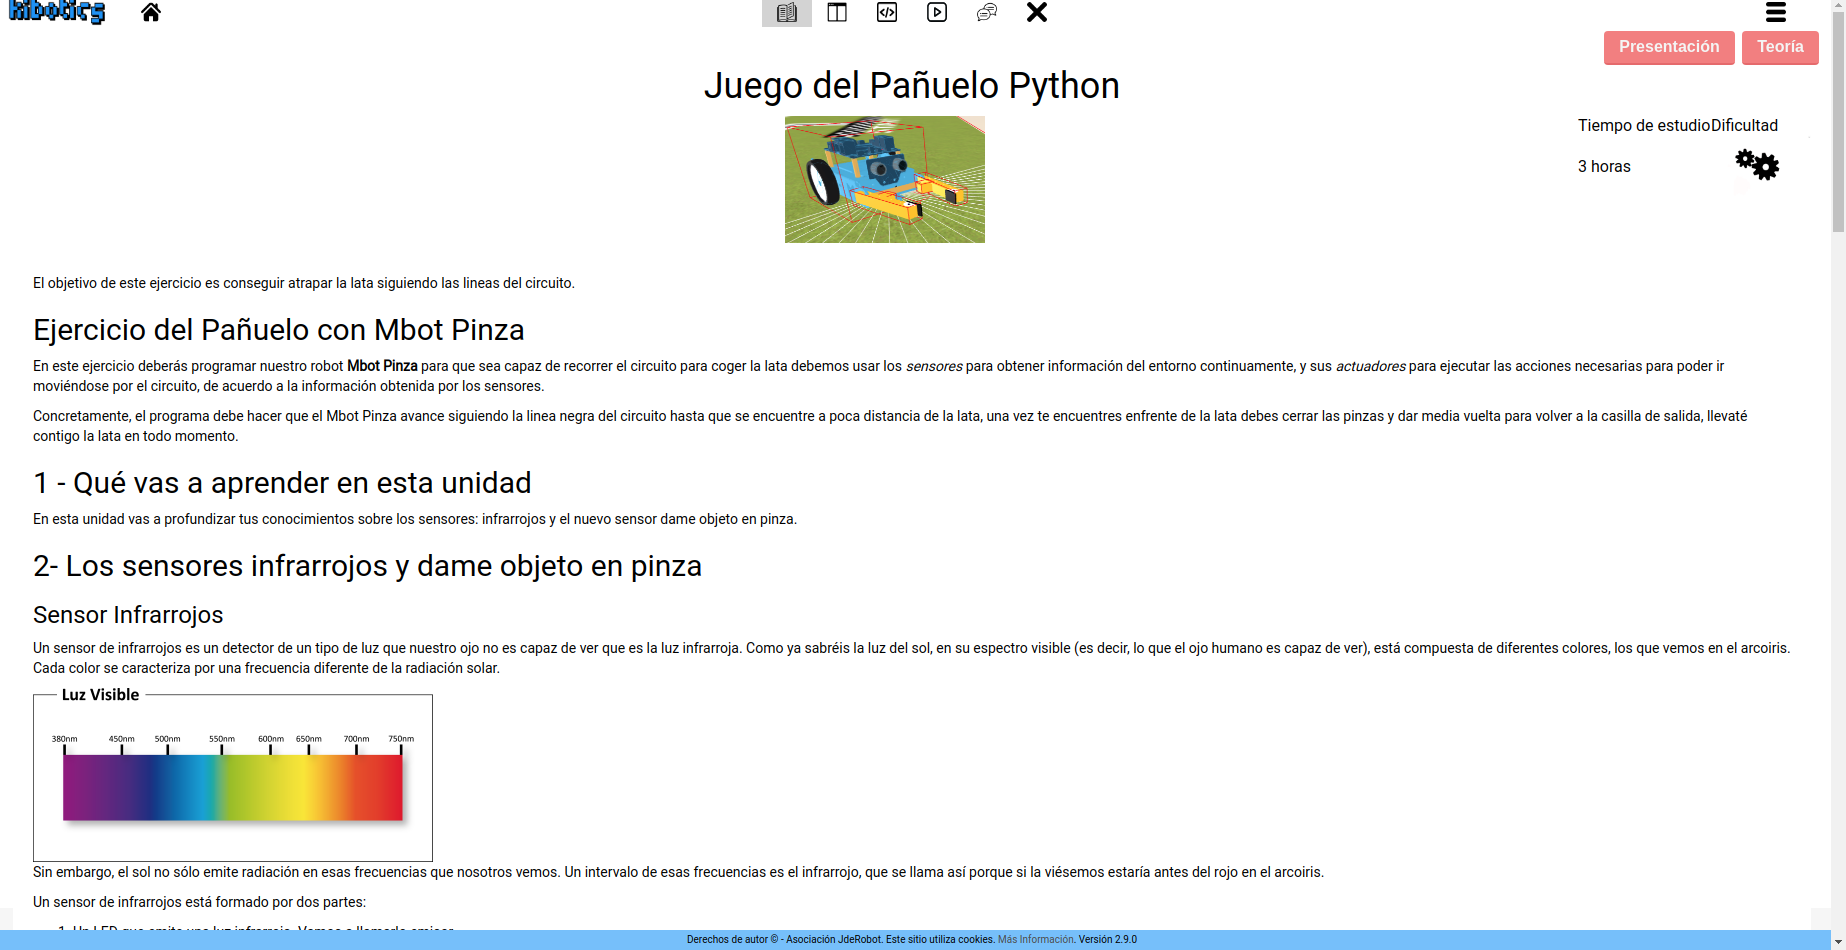
\includegraphics[width=0.8\textwidth, height=0.4\textwidth]{chapters/images/teoriag1.png}
    \caption{Página de teoría enunciado y requisitos}
    \label{fig:my_label}
\end{figure}
\begin{figure}[H]
    \centering
    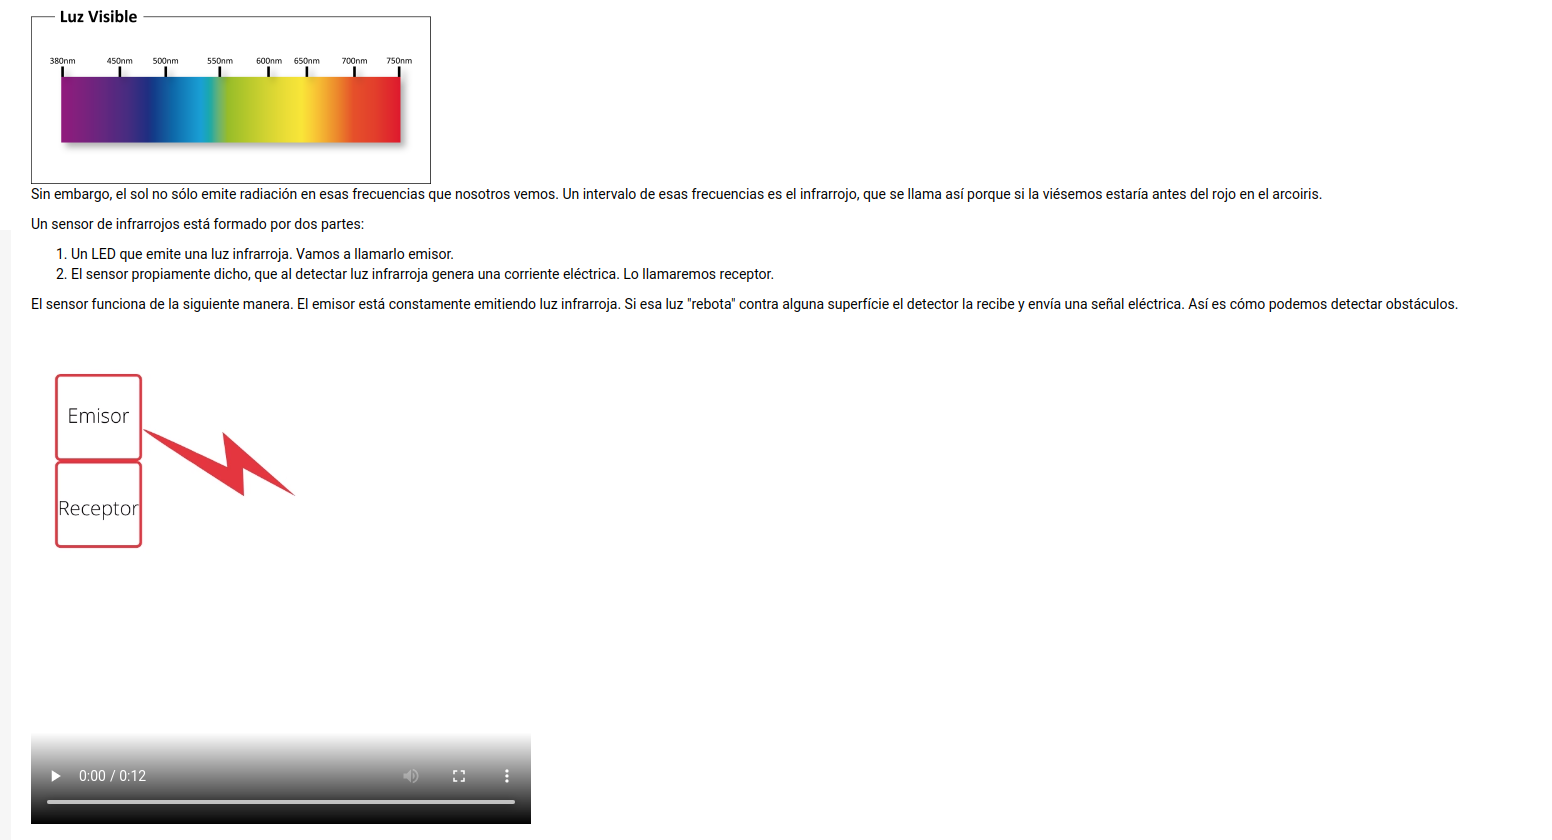
\includegraphics[width=0.8\textwidth, height=0.4\textwidth]{chapters/images/teoriag2.png}
    \caption{Teoría infrarrojos}
    \label{fig:my_label}
\end{figure}
\begin{figure}[H]
    \centering
    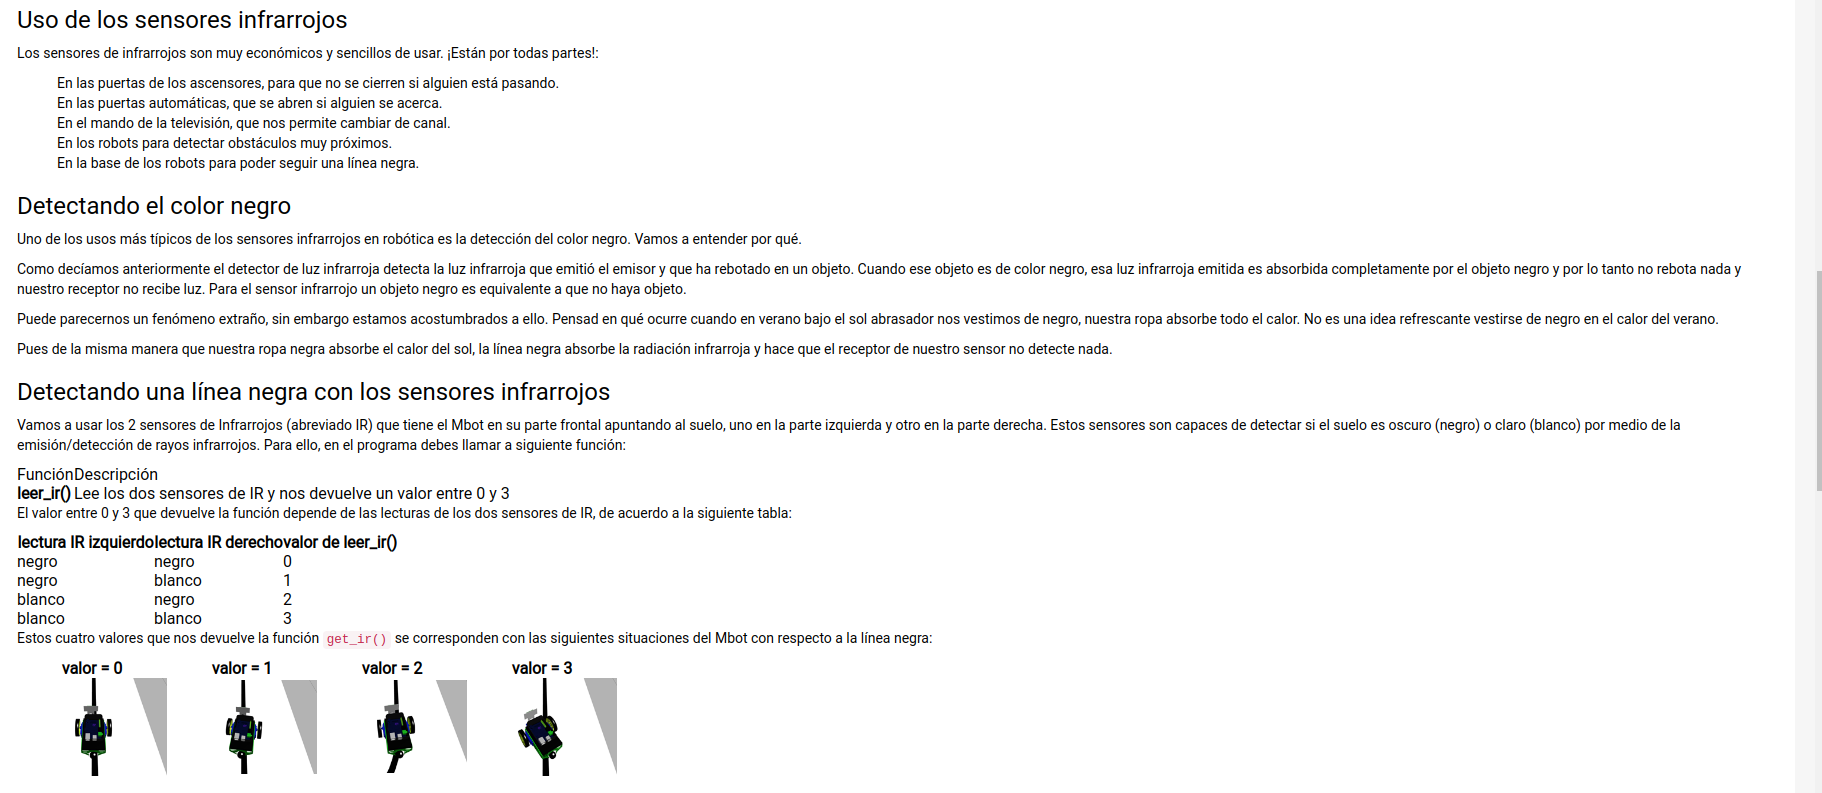
\includegraphics[width=0.8\textwidth, height=0.4\textwidth]{chapters/images/teoriag3.png}
    \caption{Teoría sensor infrarrojos}
    \label{fig:my_label}
\end{figure}

\begin{figure}[H]
    \centering
    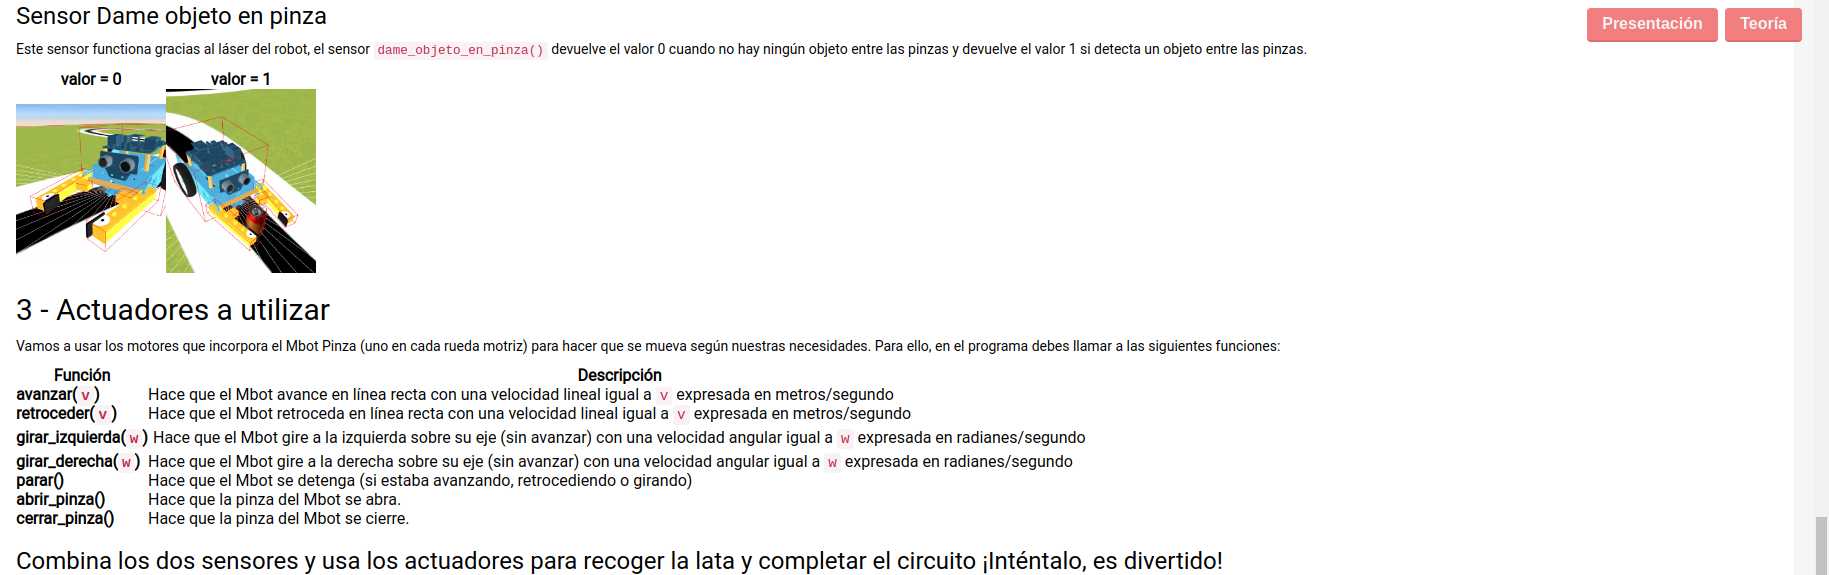
\includegraphics[width=0.8\textwidth, height=0.4\textwidth]{chapters/images/teoriag4python.png}
    \caption{Teroría sensores y actuadores en Python}
    \label{fig:my_label}
\end{figure}
\begin{figure}[H]
    \centering
    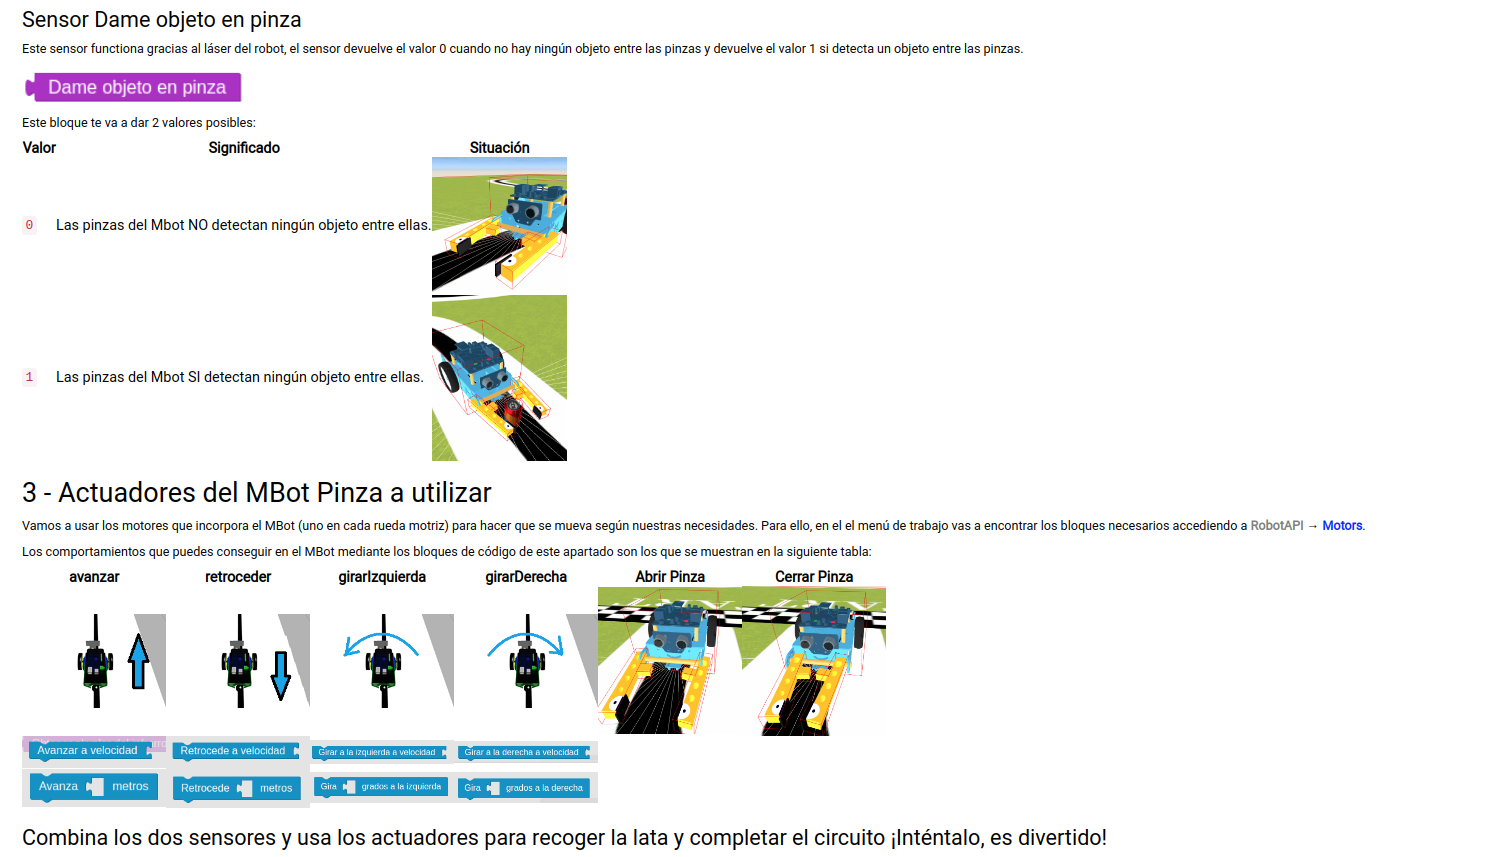
\includegraphics[width=0.8\textwidth, height=0.4\textwidth]{chapters/images/teoriag4scratch.png}
    \caption{Teroría sensores y actuadores en Python}
    \label{fig:my_label}
\end{figure}
\begin{figure}[H]
    \centering
    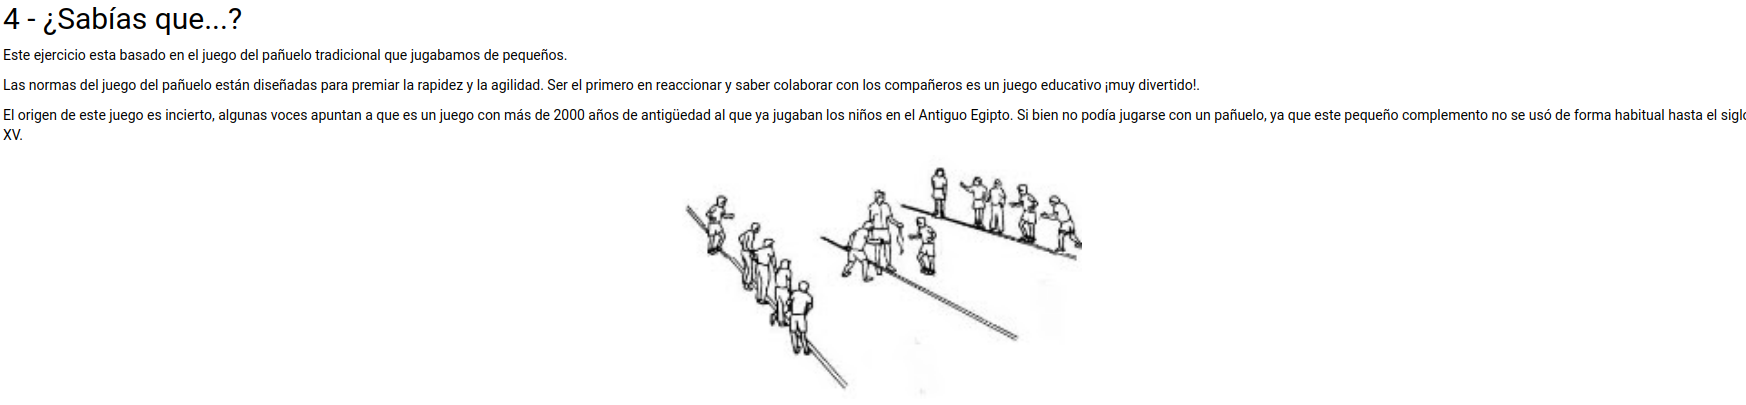
\includegraphics[width=0.8\textwidth, height=0.4\textwidth]{chapters/images/teoriag5.png}
    \caption{¿Sabías que.. ?}
    \label{fig:my_label}
\end{figure}

\section{Solución de referencia}
Este ejercicio se puede resolver de muchas formas, una de ellas es la que se muestra en la Figura 6. **para Python y para Scratch una solución posible es la que se indica en la Figura 6.** . 

\begin{figure}[H]
    \centering
    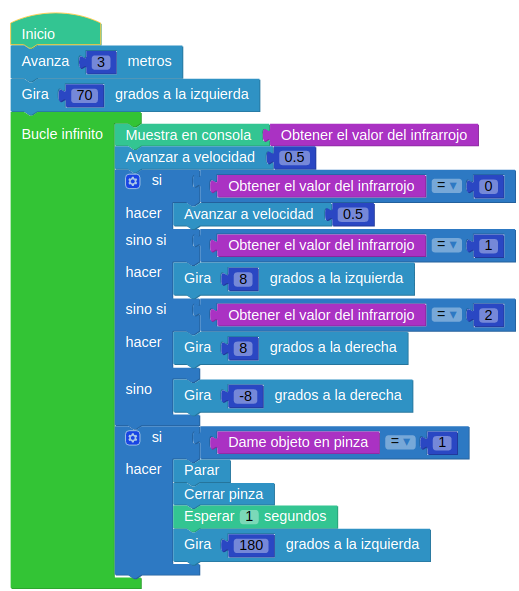
\includegraphics[width=0.7\textwidth, height=0.55\textwidth]{chapters/images/solucionpscratch.png}
    \caption{Solución en Scratch }
    \label{fig:my_label}
\end{figure}

\begin{figure}[H]
    \centering
    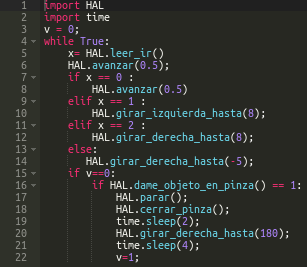
\includegraphics[width=0.7\textwidth, height=0.55\textwidth]{chapters/images/solucionppython.png}
    \caption{Solución en Python}
    \label{fig:my_label}
\end{figure}